\documentclass[]{article}
\usepackage{geometry,tikz,lipsum,amsmath,amssymb,soul,xcolor,cancel,esint}
\tikzset{every picture/.style={line width=0.75pt}} %set default line width to 0.75pt        
\numberwithin{equation}{section}

\NewDocumentCommand{\caja}{ m O{gray!40} O{gray!10} m }{
	\begin{figure}[h]
		\centering
		\begin{tikzpicture}
			\node[anchor=text, text width=\columnwidth-1.2cm, draw, rounded corners, line width=1pt, fill=#3, inner sep=5mm] (big) {\\#4};
			\node[draw, rounded corners, line width=.5pt, fill=#2, anchor=west, xshift=5mm] (small) at (big.north west) {#1};
		\end{tikzpicture}
	\end{figure}
}
\NewDocumentCommand{\indUpDown}{ O{\Lambda} O{\mu} O{\nu} }{
	{#1}^{#2}_{\ #3}
}
\NewDocumentCommand{\indDownUp}{ O{\Lambda} O{\mu} O{\nu} }{
	{#1}_{#2}^{\ #3}
}
\newcommand{\LambdaMuNu}{\indUpDown}
\newcommand{\0}{\textcolor{gray}{0}}
\newcommand{\rbf}{\mathbf{r}}
\newcommand{\ei}{\mathbf{e}_i}
\newcommand{\ej}{\mathbf{e}_j}
\newcommand{\lc}{\epsilon_{ijk}}
\newcommand{\gr}{\nabla}
\newcommand{\di}{\nabla\cdot}
\newcommand{\ro}{\nabla\times}
\newcommand{\la}{\nabla^2}
\newcommand{\rv}{\mathbf{r}}
\newcommand{\xv}{\mathbf{x}}
\newcommand{\yv}{\mathbf{y}}
\newcommand{\zv}{\mathbf{z}}
\newcommand{\xhat}{\hat{\xv}}
\newcommand{\yhat}{\hat{\yv}}
\newcommand{\zhat}{\hat{\zv}}
\newcommand{\rhat}{\hat{\rv}}
\newcommand{\that}{\hat{\mathbf{\theta}}}
\newcommand{\phat}{\hat{\mathbf{\varphi}}}
\newcommand{\rhhat}{\hat{\mathbf{\rho}}}
\newcommand{\nhat}{\hat{\mathbf{n}}}
\newcommand{\eo}{\epsilon_{0}}
\newcommand{\uo}{\mu_{0}}
\newcommand{\ke}{\frac{1}{4\pi\eo}}
\newcommand{\rdif}{\rv - \rv'}
\newcommand{\pd}[2]{\dfrac{\partial #1}{\partial #2}}
\newcommand{\lpd}[2]{\partial #1/\partial #2}
\newcommand{\td}[2]{\dfrac{d #1}{d #2}}
\newcommand{\ltd}[2]{d #1/d #2}
\newcommand{\n}[1]{\mathbf{#1}}
%opening
\title{Ejercicio 2b}
\author{Simon Fonseca}

\begin{document}
	\maketitle
	\begin{figure}[h!]
		\centering
		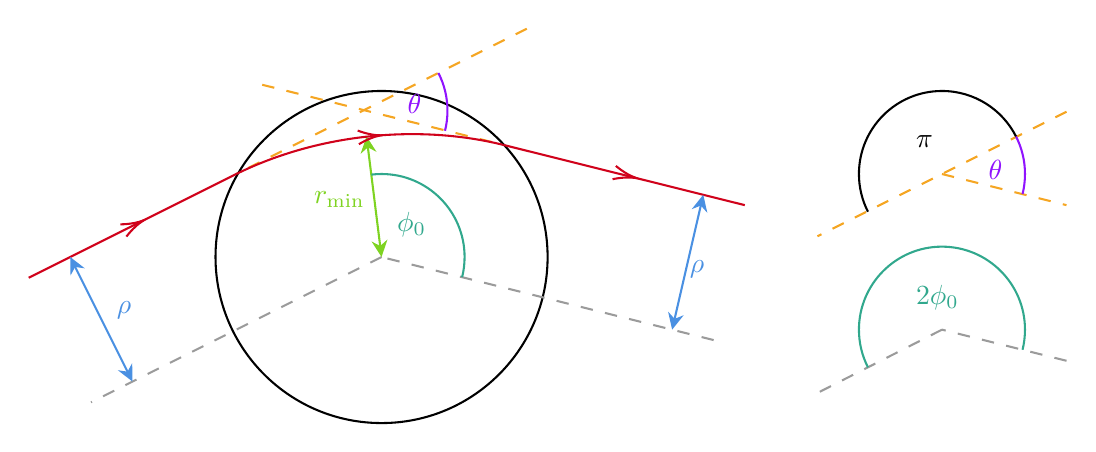
\begin{tikzpicture}[x=0.75pt,y=0.75pt,yscale=-1,xscale=1]
			%uncomment if require: \path (0,300); %set diagram left start at 0, and has height of 300
			
			%Straight Lines [id:da9671167646059478] 
			\draw [color={rgb, 255:red, 245; green, 166; blue, 35 }  ,draw opacity=1 ] [dash pattern={on 4.5pt off 4.5pt}]  (152.5,52) -- (268.75,81) ;
			%Straight Lines [id:da605209421047459] 
			\draw [color={rgb, 255:red, 245; green, 166; blue, 35 }  ,draw opacity=1 ] [dash pattern={on 4.5pt off 4.5pt}]  (280,25) -- (140,95) ;
			%Shape: Circle [id:dp46211650000796345] 
			\draw   (130,135) .. controls (130,90.82) and (165.82,55) .. (210,55) .. controls (254.18,55) and (290,90.82) .. (290,135) .. controls (290,179.18) and (254.18,215) .. (210,215) .. controls (165.82,215) and (130,179.18) .. (130,135) -- cycle ;
			%Straight Lines [id:da4708428042354711] 
			\draw [color={rgb, 255:red, 208; green, 2; blue, 27 }  ,draw opacity=1 ]   (40,145) -- (140,95) ;
			\draw [shift={(95.37,117.32)}, rotate = 153.43] [color={rgb, 255:red, 208; green, 2; blue, 27 }  ,draw opacity=1 ][line width=0.75]    (10.93,-3.29) .. controls (6.95,-1.4) and (3.31,-0.3) .. (0,0) .. controls (3.31,0.3) and (6.95,1.4) .. (10.93,3.29)   ;
			%Straight Lines [id:da8821390545721265] 
			\draw [color={rgb, 255:red, 155; green, 155; blue, 155 }  ,draw opacity=1 ] [dash pattern={on 4.5pt off 4.5pt}]  (210,135) -- (70,205) ;
			%Straight Lines [id:da42576797317584303] 
			\draw [color={rgb, 255:red, 208; green, 2; blue, 27 }  ,draw opacity=1 ]   (268.75,81) -- (385,110) ;
			\draw [shift={(332.7,96.95)}, rotate = 194.01] [color={rgb, 255:red, 208; green, 2; blue, 27 }  ,draw opacity=1 ][line width=0.75]    (10.93,-3.29) .. controls (6.95,-1.4) and (3.31,-0.3) .. (0,0) .. controls (3.31,0.3) and (6.95,1.4) .. (10.93,3.29)   ;
			%Straight Lines [id:da6463238187043812] 
			\draw [color={rgb, 255:red, 74; green, 144; blue, 226 }  ,draw opacity=1 ]   (61.34,137.68) -- (88.66,192.32) ;
			\draw [shift={(90,195)}, rotate = 243.43] [fill={rgb, 255:red, 74; green, 144; blue, 226 }  ,fill opacity=1 ][line width=0.08]  [draw opacity=0] (8.04,-3.86) -- (0,0) -- (8.04,3.86) -- (5.34,0) -- cycle    ;
			\draw [shift={(60,135)}, rotate = 63.43] [fill={rgb, 255:red, 74; green, 144; blue, 226 }  ,fill opacity=1 ][line width=0.08]  [draw opacity=0] (8.04,-3.86) -- (0,0) -- (8.04,3.86) -- (5.34,0) -- cycle    ;
			%Straight Lines [id:da3925059733644658] 
			\draw [color={rgb, 255:red, 155; green, 155; blue, 155 }  ,draw opacity=1 ] [dash pattern={on 4.5pt off 4.5pt}]  (370,175) -- (210,135) ;
			%Straight Lines [id:da029139227709992777] 
			\draw [color={rgb, 255:red, 74; green, 144; blue, 226 }  ,draw opacity=1 ]   (364.33,107.92) -- (350.67,167.08) ;
			\draw [shift={(350,170)}, rotate = 282.99] [fill={rgb, 255:red, 74; green, 144; blue, 226 }  ,fill opacity=1 ][line width=0.08]  [draw opacity=0] (8.04,-3.86) -- (0,0) -- (8.04,3.86) -- (5.34,0) -- cycle    ;
			\draw [shift={(365,105)}, rotate = 102.99] [fill={rgb, 255:red, 74; green, 144; blue, 226 }  ,fill opacity=1 ][line width=0.08]  [draw opacity=0] (8.04,-3.86) -- (0,0) -- (8.04,3.86) -- (5.34,0) -- cycle    ;
			%Straight Lines [id:da17580479289122752] 
			\draw [color={rgb, 255:red, 126; green, 211; blue, 33 }  ,draw opacity=1 ]   (203.12,79.8) -- (209.63,132.02) ;
			\draw [shift={(210,135)}, rotate = 262.9] [fill={rgb, 255:red, 126; green, 211; blue, 33 }  ,fill opacity=1 ][line width=0.08]  [draw opacity=0] (8.04,-3.86) -- (0,0) -- (8.04,3.86) -- (5.34,0) -- cycle    ;
			\draw [shift={(202.75,76.83)}, rotate = 82.9] [fill={rgb, 255:red, 126; green, 211; blue, 33 }  ,fill opacity=1 ][line width=0.08]  [draw opacity=0] (8.04,-3.86) -- (0,0) -- (8.04,3.86) -- (5.34,0) -- cycle    ;
			%Curve Lines [id:da8866221175141287] 
			\draw [color={rgb, 255:red, 208; green, 2; blue, 27 }  ,draw opacity=1 ]   (140,95) .. controls (180.25,75.25) and (228.5,71) .. (268.75,81) ;
			\draw [shift={(209.68,76.37)}, rotate = 174.78] [color={rgb, 255:red, 208; green, 2; blue, 27 }  ,draw opacity=1 ][line width=0.75]    (10.93,-3.29) .. controls (6.95,-1.4) and (3.31,-0.3) .. (0,0) .. controls (3.31,0.3) and (6.95,1.4) .. (10.93,3.29)   ;
			%Shape: Arc [id:dp022684491761803205] 
			\draw  [draw opacity=0] (237.4,46.34) .. controls (240.18,51.79) and (241.75,57.96) .. (241.75,64.5) .. controls (241.75,67.84) and (241.34,71.08) .. (240.57,74.18) -- (201.75,64.5) -- cycle ; \draw  [color={rgb, 255:red, 144; green, 19; blue, 254 }  ,draw opacity=1 ] (237.4,46.34) .. controls (240.18,51.79) and (241.75,57.96) .. (241.75,64.5) .. controls (241.75,67.84) and (241.34,71.08) .. (240.57,74.18) ;  
			%Shape: Arc [id:dp0071782192266609535] 
			\draw  [draw opacity=0] (205.12,95.29) .. controls (206.72,95.1) and (208.35,95) .. (210,95) .. controls (232.09,95) and (250,112.91) .. (250,135) .. controls (250,138.34) and (249.59,141.58) .. (248.82,144.68) -- (210,135) -- cycle ; \draw  [color={rgb, 255:red, 49; green, 168; blue, 141 }  ,draw opacity=1 ] (205.12,95.29) .. controls (206.72,95.1) and (208.35,95) .. (210,95) .. controls (232.09,95) and (250,112.91) .. (250,135) .. controls (250,138.34) and (249.59,141.58) .. (248.82,144.68) ;  
			%Straight Lines [id:da8616161522287311] 
			\draw [color={rgb, 255:red, 245; green, 166; blue, 35 }  ,draw opacity=1 ] [dash pattern={on 4.5pt off 4.5pt}]  (480,95) -- (540,110) ;
			%Straight Lines [id:da27908315426377883] 
			\draw [color={rgb, 255:red, 245; green, 166; blue, 35 }  ,draw opacity=1 ] [dash pattern={on 4.5pt off 4.5pt}]  (540,65) -- (420,125) ;
			%Shape: Arc [id:dp3181349344037647] 
			\draw  [draw opacity=0] (515.65,76.84) .. controls (518.43,82.29) and (520,88.46) .. (520,95) .. controls (520,98.34) and (519.59,101.58) .. (518.82,104.68) -- (480,95) -- cycle ; \draw  [color={rgb, 255:red, 144; green, 19; blue, 254 }  ,draw opacity=1 ] (515.65,76.84) .. controls (518.43,82.29) and (520,88.46) .. (520,95) .. controls (520,98.34) and (519.59,101.58) .. (518.82,104.68) ;  
			%Straight Lines [id:da30303795588362215] 
			\draw [color={rgb, 255:red, 155; green, 155; blue, 155 }  ,draw opacity=1 ] [dash pattern={on 4.5pt off 4.5pt}]  (480,170) -- (420,200.5) ;
			%Straight Lines [id:da7995818259242062] 
			\draw [color={rgb, 255:red, 155; green, 155; blue, 155 }  ,draw opacity=1 ] [dash pattern={on 4.5pt off 4.5pt}]  (540,185) -- (480,170) ;
			%Shape: Arc [id:dp1576050398493577] 
			\draw  [draw opacity=0] (444.35,188.16) .. controls (441.57,182.71) and (440,176.54) .. (440,170) .. controls (440,147.91) and (457.91,130) .. (480,130) .. controls (502.09,130) and (520,147.91) .. (520,170) .. controls (520,173.34) and (519.59,176.58) .. (518.82,179.68) -- (480,170) -- cycle ; \draw  [color={rgb, 255:red, 49; green, 168; blue, 141 }  ,draw opacity=1 ] (444.35,188.16) .. controls (441.57,182.71) and (440,176.54) .. (440,170) .. controls (440,147.91) and (457.91,130) .. (480,130) .. controls (502.09,130) and (520,147.91) .. (520,170) .. controls (520,173.34) and (519.59,176.58) .. (518.82,179.68) ;  
			%Shape: Arc [id:dp12975946624919743] 
			\draw  [draw opacity=0] (444.35,113.16) .. controls (441.57,107.71) and (440,101.54) .. (440,95) .. controls (440,72.91) and (457.91,55) .. (480,55) .. controls (495.55,55) and (509.03,63.88) .. (515.65,76.84) -- (480,95) -- cycle ; \draw  [color={rgb, 255:red, 0; green, 0; blue, 0 }  ,draw opacity=1 ] (444.35,113.16) .. controls (441.57,107.71) and (440,101.54) .. (440,95) .. controls (440,72.91) and (457.91,55) .. (480,55) .. controls (495.55,55) and (509.03,63.88) .. (515.65,76.84) ;  
			
			% Text Node
			\draw (81,155) node [anchor=north west][inner sep=0.75pt]  [color={rgb, 255:red, 74; green, 144; blue, 226 }  ,opacity=1 ] [align=left] {$\displaystyle \rho $};
			% Text Node
			\draw (357,135) node [anchor=north west][inner sep=0.75pt]  [color={rgb, 255:red, 74; green, 144; blue, 226 }  ,opacity=1 ] [align=left] {$\displaystyle \rho $};
			% Text Node
			\draw (176,102) node [anchor=north west][inner sep=0.75pt]  [color={rgb, 255:red, 126; green, 211; blue, 33 }  ,opacity=1 ] [align=left] {$\displaystyle r_{\mathrm{min}}$};
			% Text Node
			\draw (221,55) node [anchor=north west][inner sep=0.75pt]  [color={rgb, 255:red, 144; green, 19; blue, 254 }  ,opacity=1 ] [align=left] {$\displaystyle \theta $};
			% Text Node
			\draw (216,112) node [anchor=north west][inner sep=0.75pt]  [color={rgb, 255:red, 49; green, 168; blue, 141 }  ,opacity=1 ] [align=left] {$\displaystyle \phi _{0}$};
			% Text Node
			\draw (501,87) node [anchor=north west][inner sep=0.75pt]  [color={rgb, 255:red, 144; green, 19; blue, 254 }  ,opacity=1 ] [align=left] {$\displaystyle \theta $};
			% Text Node
			\draw (466,147) node [anchor=north west][inner sep=0.75pt]  [color={rgb, 255:red, 49; green, 168; blue, 141 }  ,opacity=1 ] [align=left] {$\displaystyle 2\phi _{0}$};
			% Text Node
			\draw (466,75) node [anchor=north west][inner sep=0.75pt]   [align=left] {$\displaystyle \pi $};
		\end{tikzpicture}
	\end{figure}
	
	From part (a), we found the potential:
	$$U(r) = \begin{cases} 2E_0\left(1 - \frac{R}{r}\right), & r < R \\ 0, & r \geq R \end{cases}$$
	
	Now we're shooting particles at a different energy $E$ and need to find the scattering cross-section.
	
	The scattering angle $\theta$ relates to the angle $\phi_0$ through:
	$$\theta = \pi - 2\phi_0$$
	
	where $\phi_0$ is the angle from the initial direction to the point of closest approach.
	
	The angle $\phi_0$ comes from integrating the trajectory:
	$$\phi_0 = \int_{\infty}^{r_{min}} \frac{M \, dr}{mr^2\sqrt{\frac{2}{m}(E - U(r)) - \frac{M^2}{m^2r^2}}}$$
	where $M = m v_\infty \rho$ and $E = \frac{1}{2} m v_\infty^2$.
	
	This splits into two regions because U(r) has two forms:
	
	$$\phi_0 = \int^{R}_{r_{min}} \frac{\rho/r^2 \, dr}{\sqrt{1 - \frac{4E_0}{mv^2_\infty}\left(1 - \frac{R}{r}\right) - \frac{\rho^2}{r^2}}} + \int^{\infty}_{R} \frac{\rho/r^2 \, dr}{\sqrt{1 - \frac{\rho^2}{r^2}}}$$
	
	The second integral (outside the potential) is simple:
	$$\int^{\infty}_{R} \frac{\rho/r^2 \, dr}{\sqrt{1 - \frac{\rho^2}{r^2}}} = \arctan\left(\frac{\rho}{\sqrt{R^2 - \rho^2}}\right)$$
		
	Inside the potential region, notice:
	$$U(r) = 2E_0 - \frac{2E_0 R}{r}$$
	
	The constant $2E_0$ just shifts the energy. The $-\frac{2E_0 R}{r}$ term is exactly like a Coulomb potential with $\alpha = 2E_0R$.
	
	So inside $r < R$, the trajectory is a conic section (like Kepler orbits):
	$$\frac{p}{r} = 1 + e\cos\phi$$
	
	with parameters:
	$$p = \frac{M^2}{2mE_0R}, \quad e = \sqrt{1 + \frac{2(E - 2E_0)M^2}{4mE_0^2R^2}}$$
	
	meaning that, at the closest approach $(r=r_{min})$, the radial velocity is zero, which occurs when $\phi=0$ (by our choice of coordinates). So:
	
	$$\frac{p}{r_{min}} = 1 + e \Rightarrow r_{min} = \frac{p}{1 + e}$$
	
	
	The integral inside the potential region goes from $r_{min}$ to $R$:
	
	$$\phi_0^{(inside)} = \int_{r_{min}}^{R} \frac{\rho/r^2 \, dr}{\sqrt{1 - \frac{4E_0}{mv^2_\infty}\left(1 - \frac{R}{r}\right) - \frac{\rho^2}{r^2}}}$$
	
	Since we know the trajectory is a conic section with $\frac{p}{r} = 1 + e\cos\phi$, we can change variables from $r$ to $\phi$:
	
	From $r = \frac{p}{1 + e\cos\phi}$, we get:
	$$dr = \frac{pe\sin\phi}{(1 + e\cos\phi)^2} d\phi$$
	
	The integral becomes:
	$$\phi_0^{(inside)} = \int_{0}^{\phi_R} d\phi$$
	
	where $\phi_R$ is the angle when the particle exits at $r = R$:
	$$\frac{p}{R} = 1 + e\cos\phi_R$$
	
	So:
	$$\cos\phi_R = \frac{1}{e}\left(\frac{p}{R} - 1\right)$$
	
	Outside the potential:
	$$\phi_0^{(outside)} = \arctan\left(\frac{\rho}{\sqrt{R^2 - \rho^2}}\right)$$
	
	This is the additional angle traveled from $r = R$ to $r = \infty$ along a straight line.
	
	Total $\phi_0$
	
	$$\phi_0 = \phi_R + \arctan\left(\frac{\rho}{\sqrt{R^2 - \rho^2}}\right)$$
	
	where:
	$$\phi_R = \arccos\left[\frac{1}{e}\left(\frac{p}{R} - 1\right)\right]$$
	
	Now substitute back, you get:
	$$\tan\phi_0 = \frac{\rho(mv^2_\infty - 2E_0)}{2E_0\sqrt{R^2 - \rho^2}}$$
	
	Since $\phi_0 = \frac{\pi - \theta}{2}$, we have $\tan\phi_0 = \cot(\theta/2)$:
	
	$$\rho = \frac{2E_0 R \cot(\theta/2)}{\sqrt{4E_0^2 + m^2v^4 - 4E_0 mv^2 + 4E_0^2\cot^2(\theta/2)}}$$
	
	The differential cross-section is:
	$$\frac{d\sigma}{d\Omega} = \frac{1}{2\pi\sin\theta} \cdot 2\pi\rho \left|\frac{d\rho}{d\theta}\right| = \frac{1}{\sin\theta}\rho\left|\frac{d\rho}{d\theta}\right|$$
	
	After computing $\frac{d\rho}{d\theta}$, you get:
	
	$$\boxed{\frac{d\sigma}{d\Omega} = \frac{E_0^2 R^2}{(E_0 - E)^2}\left[E_0^2\cos^2(\theta/2) + (E_0 - E)^2\sin^2(\theta/2)\right]^{-2}}$$
	
	where $E = \frac{1}{2}mv^2$.
	
	
	As $E \to E_0$:
	$$\frac{d\sigma}{d\Omega} \to \frac{E_0^2 R^2}{(E_0 - E)^2 \cdot E_0^4\cos^4(\theta/2)} \sim \frac{R^2}{(E_0 - E)^2\cos^4(\theta/2)}$$
	
	The cross-section diverges. This makes physical sense: at $E = E_0$, all particles with $\rho < R$ scatter to exactly \(\theta = \pi\), creating a singularity.
\end{document}

